\begin{frame}
	\frametitle{Modelo de Produ\c c\~ao}
	\begin{center}
		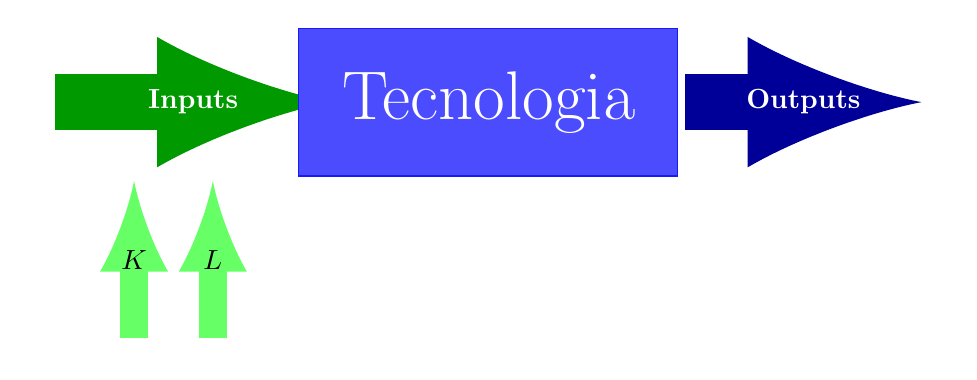
\begin{tikzpicture}[
			scale = 1,
			every node/.style ={scale =1}
		]

		\onslide<1->{
			\draw[->, >=latex,draw=green!60!white,fill=green!20!white, line width=10pt] (0,0) to node[black]{$K$} (0,2);
			\draw[->, >=latex,draw=green!60!white,fill=green!20!white, line width=10pt] (1,0) to node[black]{$L$} (1,2);
		}

		\onslide<2->{
			\draw[->, >=latex,green!60!black,line width=20pt] (-1,3) to node[white]{\textbf{Inputs}} (2.5,3);
		}

		\onslide<3->{
			\node[draw=blue!90!white,rectangle,fill=blue!70!white,inner sep=5.5mm,text=white] at (4.5,3) {\Huge Tecnologia} ;
		}

		\onslide<4->{
			\draw[->, >=latex,blue!60!black,line width=20pt] (7,3) to node[white]{\textbf{Outputs}} (10,3);		
		}

		\end{tikzpicture}
	\end{center}

	\onslide<5->{
		Uma unidade produtiva (produtor) contrata inputs no mercado de fatores e, usando uma tecnologia, transforma-os em \emph{output}
	}
\end{frame}

\begin{frame}
	\frametitle{Modelo de Produ\c c\~ao}
	S\~ao escolhas da empresa:
	\begin{itemize}
		\item Quantidade de cada \emph{input} a contratar, em fun\c c\~ao dos respectivos pre\c cos de mercado
		\item Quantidade de \emph{output} a produzir, o que depende das condi\c c\~oes de mercado em que a unidade produtiva est\'a inserida, e da tecnologia instalada.
	\end{itemize}
\end{frame}

\begin{frame}
	\frametitle{Linguagem}
	\begin{itemize}
		\item \textbf{Fun\c c\~ao de Produ\c c\~ao:} Rela\c c\~ao entre quantidade de \emph{inputs} e quantidade de \emph{output} que a partir deles se obt\'em, dada uma tecnologia:\[F(K,L)=Q\] \pause
		\item \textbf{Fun\c c\~ao Custos:} rela\c c\~ao entre custos de contrata\c c\~ao de \emph{inputs} e quantidade de \emph{output} que a partir deles se obt\'em, dada uma tecnologia:\[CT=C(Q)\]
	\end{itemize}
\end{frame}

\begin{frame}
	\frametitle{Fun\c c\~ao de Produ\c c\~ao}
	\begin{itemize}
		\item Uma fun\c c\~ao de produ\c c\~ao mostra o produto m\'aximo que se pode obter atrav\'es de combina\c c\~oes alternativas de factores produtivos, dada uma certa tecnologia.
		\item Pressup\~oe-se efici\^encia na utiliza\c c\~ao de recursos...
	\end{itemize}
\end{frame}

\begin{frame}
	\frametitle{Curto Prazo - Longo Prazo}
	\begin{itemize}
		\item Uma empresa tem de decidir que quantidade de produto vai fabricar, a localiza\c c\~ao do estabelecimento, quais os equipamentos a instalar, quanto pessoal deve contratar, etc...\pause
		\item As escolhas/decis\~oes da empresa s\~ao realizadas em per\'iodos de tempo diferentes, porque, por exemplo, \'e mais r\'apido contratar trabalhadores do que adquirir instala\c c\~oes.
	\end{itemize}
\end{frame}

\begin{frame}
	\frametitle{Curto Prazo (conceito)}
	O Curto Prazo \'e um periodo de tempo suficientemente curto, para que a empresa n\~ao consiga modificar a quantidade contratada de, pelo menos, um factor produtivo (factor fixo)
	
	\vspace{0.2cm}

	Normalmente, considera-se que o Capital est\'a fixo a curto prazo
\end{frame}

\begin{frame}
	\frametitle{Longo Prazo (conceito)}
	\begin{itemize}
		\item O Longo-Prazo \'e um per\'iodo de tempo suficientemente longo, para que a quantidade contratada de todos os factores produtivos possa ser alterada.
		\item \'E neste contexto que se enquadram planifica\c c\~oes de produ\c c\~ao para o futuro: \'area de produ\c c\~ao, linhas de produto, maquinara/tecnologia...
	\end{itemize}
\end{frame}

\begin{frame}
	\frametitle{``Quanto Tempo tem o Tempo?''}
	\begin{itemize}
		\item Longo-Prazo e Curto-Prazo s\~ao apenas conceitos...
		\item A quantidade de tempo necess\'aria para considerar que esse per\'iodo \'e curto-prazo ou longo-prazo depende de cada sector de atividade...
	\end{itemize}

	Ex. um m\^es pode ser o suficiente para mudar completamente a maquinaria de uma f\'abrica t\^extil, mas n\~ao ser\'a tempo suficiente para o fazer numa f\'abrica de microcomponentes eletr\'onicas... o ``longo-prazo'', nalguns sectores, pode ``demorar mais tempo'' do que noutros...
\end{frame}

\begin{frame}
	\frametitle{Factores Fixos e Factores Vari\'aveis}
	\begin{itemize}
		\item \textbf{Factores fixos} s\~ao \emph{inputs} cuja quantidade n\~ao varia no curto prazo
		\item \textbf{Factores vari\'aveis} s\~ao \emph{inputs} cuja quantidade pode ser alterada no curto prazo
	\end{itemize}

	\underline{Nos modelos seguintes, considera-se $L$ vari\'avel e $K$ fixo a curto-prazo.}
\end{frame}

\begin{frame}
	\frametitle{Fun\c c\~ao de Produ\c c\~ao: Curto Prazo}
	\begin{itemize}
		\item Uma fun\c c\~ao, para ser utilizada como modelo de tecnologia (fun\c c\~ao de produ\c c\~ao) tem certas carater\'isticas, que veremos de seguida.
		\item Uma fun\c c\~ao de produ\c c\~ao a curto prazo, considera $K$ fixo num valor $\overline{K}$ pr\'e-determinado (ex\'ogeno) e $L$ \'e vari\'avel:\[F(\overline{K},L)=f(L)\]
		(curva de produto total)
	\end{itemize}
\end{frame}

\begin{frame}
	\frametitle{Rendimentos Marginais (ou Produto Marginal do Trabalho -MPL)}
	Trata-se da forma como a Produ\c c\~ao se altera $(\Delta Q)$, quando o \emph{input} vari\'avel se altera $(\Delta L)$:\[Pmg=MPL=\frac{\Delta Q}{\Delta L}\]
\end{frame}

\begin{frame}
	\frametitle{MPL}
	Produto marginal de um factor vari\'avel (o trabalho) \'e a varia\c c\~ao do produto total quando se adiciona \`a produ\c c\~ao uma unidade desse factor produtivo, \emph{c\ae teris paribus}, ou seja, mantendo constante a quantidade dos outros factores (o capital, $K$)
\end{frame}

\begin{frame}
	\frametitle{Produto M\'edio do Trabalho - APL}
	\'E a quantidade produzida, em m\'edia, por cada unidade de trabalho contratada:\[PMe = APL = \frac{Q}{L}\]
	Uma ``unidade de trabalho'' pode ser uma pessoa, grupos de pessoas, ou horas/dias/(unidade de tempo) de trabalho
\end{frame}

\begin{frame}
	\frametitle{Exemplo: rela\c c\~ao entre APL e MPL}
	\begin{center}
		{
		\renewcommand{\arraystretch}{1.2}
		\begin{tabular}{|cccc|}
			\hline
			L & F(K,L) & APL & MPL \\ \hline \hline
			0 & 0 & 0 & 0 \\
			1 & 4 & 4 & 4 \\
			2 & 14 & 7 & 10 \\
			3 & 27 & 9 & 13 \\
			\cellcolor{yellow}4 & 43 & 10.75 & 16 \\
			5 & 58 & 11.6 & 15 \\
			6 & 72 & 12 &  14 \\
			7 & 81 & 11.57 &  9 \\
			8 & 86 & 10.75 & 5 \\
			9 & 78 & 8.67 & -8 \\
			10 & 67 & 6.7 & -11 \\ \hline
		\end{tabular}
		}
	\end{center}

	\begin{tikzpicture}[remember picture, overlay]
		\draw[->,thick,green!80!black] (2.9,6.5) -| (2.5,4) node[black,midway,xshift=-2cm,yshift=-1cm]{\parbox[c]{2.75cm}{Rendimentos mg \\ crescentes}};
		\draw[->,thick,green!60!black] (2.9,3.75) -| (2.5,1.5) node[black,midway,xshift=-2cm,yshift=-1cm]{\parbox[c]{2.75cm}{Rendimentos mg \\ Decrescentes}};
		\draw[->,thick,red] (2.9,1.25) -| (2.5,0.5) node[black,midway,xshift=-2cm,yshift=-0.5cm]{\parbox[c]{2.75cm}{Rendimentos mg \\negativos}};

		\draw[->,thick,blue!70!black] (7.9,0.5) -| (8.3,2.5) node[black,midway,xshift=1.7cm,yshift=1cm]{\parbox[c]{3.1cm}{$APL>MPL$ \\ ($APL$ decrescente)}} ;
		\draw[->,thick,blue!70!black] (7.9,2.75) -| (8.3,6.5) node[black,midway,xshift=1.7cm,yshift=2cm]{\parbox[c]{3.1cm}{$APL<MPL$ \\ ($APL$ crescente)}} ;
	\end{tikzpicture}

\end{frame}

\begin{frame}
	\frametitle{Curva de Produto Total}
	\[F(K,L)\]
	\begin{center}
		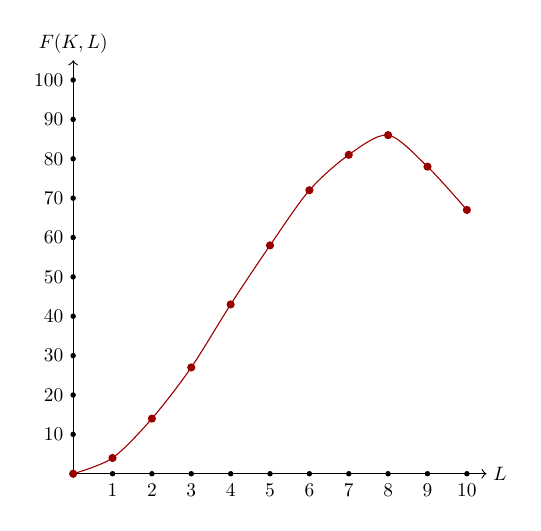
\begin{tikzpicture}[
			scale = 0.5,
			every node/.style = {scale = 0.7}
		]

		\coordinate (a) at (0,0);
		\coordinate (b) at (1,0.4);
		\coordinate (c) at (2,1.4);
		\coordinate (d) at (3,2.7);
		\coordinate (e) at (4,4.3);
		\coordinate (f) at (5,5.8);
		\coordinate (g) at (6,7.2);
		\coordinate (h) at (7,8.1);
		\coordinate (i) at (8,8.6);
		\coordinate (j) at (9,7.8);
		\coordinate (k) at (10,6.7);

		\draw[->] (-0.1,0) -- (10.5,0) node[right]{$L$};
		\draw[->] (0,-0.1) -- (0,10.5) node[above]{$F(K,L)$};

		\draw[red!60!black] plot[smooth] coordinates{(a) (b) (c) (d) (e) (f) (g) (h) (i) (j) (k)};

		\foreach \r in {1,...,10}{
			\draw (\r,0) node[circle, fill, inner sep=1,label=below:{\r}]{};
			\draw (0,\r) node[circle,fill,inner sep=1,label=left:{\r0}]{};
		}

		\foreach \r in {a,...,k}{
			\draw[red!60!black] (\r) node[circle, fill, inner sep=1.5]{};
		}

		\end{tikzpicture}
	\end{center}
\end{frame}

\begin{frame}
	\frametitle{Em Geral}
	\begin{center}
		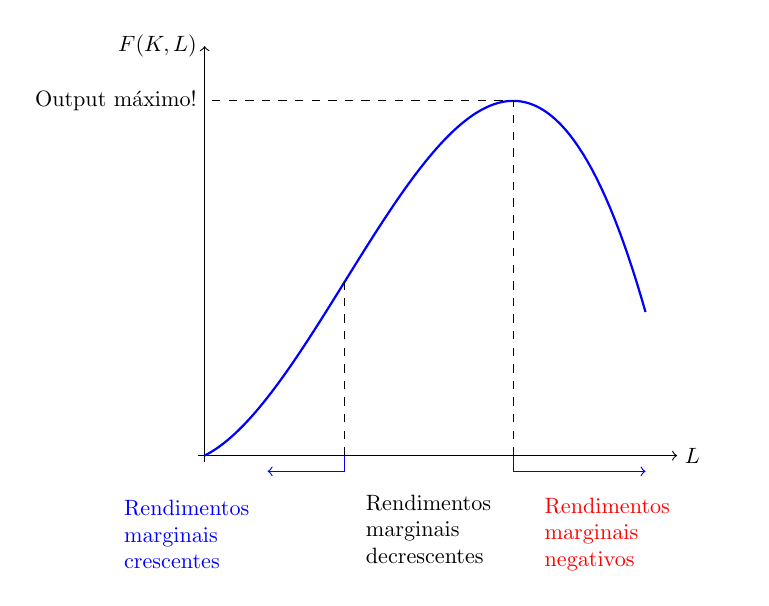
\begin{tikzpicture}[
			scale = 0.8,
			every node/.style = {scale = 0.8},
			declare function = {f(\x)=1*(\x/2)+2*(\x/2)^2-0.6*(\x/2)^3;}
			]

			\draw[->] (-0.1,0) -- (7.5,0) node[right]{$L$};
			\draw[->] (0,-0.1) -- (0,6.5) node[left]{$F(K,L)$};

			\draw[blue,thick,domain = 0:7,variable=\x,samples=100] plot (\x,{f(\x)});

			\draw[dashed] ({20/9},0) --({20/9},{f(20/9)});
			\draw[dashed] (4.89813,0) -- (4.89813,{f(4.89813)}) -- (0,{f(4.89813)})node[left]{Output m\'aximo!};

			\draw[blue,->] ({20/9},0) |- (1,-0.25)node[midway,xshift=-2cm,yshift=-1cm]{\parbox{3cm}{Rendimentos marginais\\ crescentes}};

			\draw[blue,->] (4.89813,0) |- (7,-0.25) node[red,midway,xshift=2cm,yshift=-1cm]{\parbox{3cm}{Rendimentos marginais\\ negativos}};

			\draw ({((20/9)+4.89813)/2},0) node[below,xshift=0.5cm,yshift=-0.5cm]{\parbox{3cm}{Rendimentos marginais\\ decrescentes}};

		\end{tikzpicture}
	\end{center}
\end{frame}

\begin{frame}
	\frametitle{APL e MPL no exemplo}
	\begin{columns}
		\begin{column}{0.47\textwidth}
			\begin{center}
				\begin{tikzpicture}[
					scale = 0.4,
					every node/.style = {scale = 0.4}
				]

				\coordinate (a) at (0,0);
				\coordinate (b) at (1,0.4);
				\coordinate (c) at (2,1.4);
				\coordinate (d) at (3,2.7);
				\coordinate (e) at (4,4.3);
				\coordinate (f) at (5,5.8);
				\coordinate (g) at (6,7.2);
				\coordinate (h) at (7,8.1);
				\coordinate (i) at (8,8.6);
				\coordinate (j) at (9,7.8);
				\coordinate (k) at (10,6.7);

				\draw[->] (-0.1,0) -- (10.5,0) node[right]{$L$};
				\draw[->] (0,-0.1) -- (0,10.5) node[above]{$F(K,L)$};

				\draw[blue!60!black] plot[smooth] coordinates{(a) (b) (c) (d) (e) (f) (g) (h) (i) (j) (k)};

				\foreach \r in {1,...,10}{
					\draw (\r,0) node[circle, fill, inner sep=1,label=below:{\r}]{};
					\draw (0,\r) node[circle,fill,inner sep=1,label=left:{\r0}]{};
				}

				\foreach \r in {a,...,k}{
					\draw[red!60!black] (\r) node[circle, fill, inner sep=1.5]{};
				}

				\only<2>{
					\draw[thick] (e) -- (4,0);
				}

				\only<3>{
					\draw[thick] (i) ++ (0.4,0) node[above]{$Q_{max} (MPL=0)$} -- (8.4,0);
				}

				\only<4>{
					\draw[thick] (g) ++ (0.5,0.5) -- (6.5,0);
				}

				\end{tikzpicture}
			\end{center}
			{\color{blue!60!black} Output}
		\end{column}
		\begin{column}{0.47\textwidth}
			\begin{center}
				\begin{tikzpicture}[
					scale = 0.4,
					every node/.style = {scale = 0.4}
				]

				\coordinate (a) at (0,{4*0});
				\coordinate (b) at (1,{4*0.4});
				\coordinate (c) at (2,{4*0.7});
				\coordinate (d) at (3,{4*0.9});
				\coordinate (e) at (4,{4*1.075});
				\coordinate (f) at (5,{4*1.16});
				\coordinate (g) at (6,{4*1.2});
				\coordinate (h) at (7,{4*1.157});
				\coordinate (i) at (8,{4*1.075});
				\coordinate (j) at (9,{4*0.867});
				\coordinate (k) at (10,{4*0.67});

				\coordinate (l) at (0,{4*0});
				\coordinate (m) at (1,{4*0.4});
				\coordinate (n) at (2,{4*1});
				\coordinate (o) at (3,{4*1.3});
				\coordinate (p) at (4,{4*1.6});
				\coordinate (q) at (5,{4*1.5});
				\coordinate (r) at (6,{4*1.4});
				\coordinate (s) at (7,{4*0.9});
				\coordinate (t) at (8,{4*0.5});
				\coordinate (u) at (9,{4*-0.8});
				\coordinate (v) at (10,{4*-1.1});

				\draw[->] (-0.1,0) -- (10.5,0) node[right]{$L$};
				\draw[->] (0,-5) -- (0,8) node[above]{$APL,AML$};

				\draw[red!60!black] plot[smooth] coordinates{(a) (b) (c) (d) (e) (f) (g) (h) (i) (j) (k)};
				\draw[green!60!black] plot[smooth] coordinates{(l) (m) (n) (o) (p) (q) (r) (s) (t) (u) (v)};

				\foreach \r in {1,...,10}{
					\draw (\r,0) node[circle, fill, inner sep=1,label=below:{\r}]{};
				}

				\foreach \r in {-12,...,17}{
					\draw (0,{\r*0.4}) node[circle,fill,inner sep=1,label=left:{\r}]{};
				}

				\foreach \r in {a,...,k}{
					\draw[red!60!black] (\r) node[circle, fill, inner sep=1.5]{};
				}

				\foreach \r in {l,...,v}{
					\draw[green!60!black] (\r) node[circle, fill, inner sep=1.5]{};
				}

				\only<2>{
					\draw[thick] (p) -- (4,0);
				}

				\only<3>{
					\draw[thick] (i) ++ (0.4,0)node[above]{$MPL_{max}$} -- (8.4,0);
				}

				\only<4>{
					\draw[thick] (r) ++ (0.5,0)node[above right]{$APL_{max} (APL=MPL)$} -- (6.5,0);
				}

				\end{tikzpicture}
			\end{center}
			{\color{red!60!black} APL}, {\color{green!60!black} MPL}
		\end{column}
	\end{columns}
\end{frame}